\
\
\
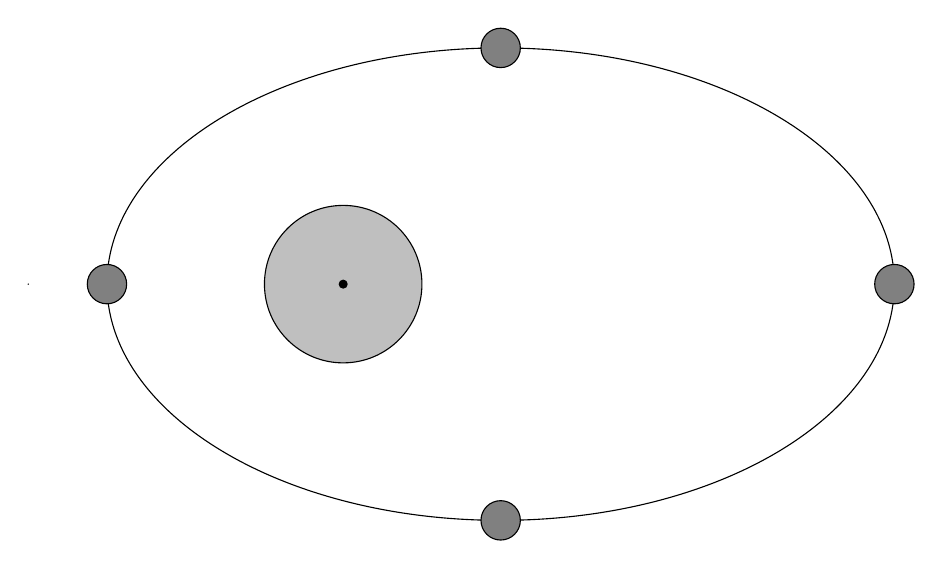
\begin{tikzpicture}
\draw (0,0) circle (0.00001cm);
\filldraw[fill = lightgray, draw = black] (4,0) circle (1cm);
\filldraw (4,0) circle (0.05cm);
\draw (6,0) ellipse (5cm and 3 cm);
\filldraw[fill = gray, draw = black] (1,0) circle (0.25cm);
\filldraw[fill = gray, draw = black] (11,0) circle (0.25cm);
\filldraw[fill = gray, draw = black] (6,3) circle (0.25cm);
\filldraw[fill = gray, draw = black] (6,-3) circle (0.25cm);
\end{tikzpicture}
\begin{center}
(Figure 7.3.1)
\end{center}
\
Kepler’s Laws of gravitation truly are not that special and are mainly taught for historical reasons. They can be derived from Newton’s Laws alone. Nonetheless, they are very interesting.

The first law is a proclamation that planets orbit the sun in elliptical orbits with the sun at one focus of the ellipse. If you are not sure about the definition of an ellipse, I recommend you read up about conic slices as they turn out to be quite crucial in describing the orbits of planets. This is not entirely true because Newton’s Laws are not a complete description of gravity. The planets orbit the sun in a sort of helix that when you view from above, appears to make an elliptical orbit. From year to year this transition may be minimal, but over a long time, this effect becomes significant. I will not present the proof of this, but I do recommend you look at a 3Blue1Brown video on his youtube channel and on the minutephysics channel where they talk about this topic. 

The second of Kepler’s Laws tells that if you draw a line from a planet orbiting the sun to the sun and calculate the area that this line sweeps out in a time t, that this area will be the same regardless of the part of the orbit that the planet is in. Graphically, this is represented in Fig. 7.3.1. I will not attempt to prove this to you either because it requires some more sophisticated mathematics but the physical principle used to prove this involves the conservation of angular momentum. 

The last of Kepler’s Laws we will prove in a special case. The third law states that the square of the period for a planet orbiting a star is proportional to the third power of the length of the semi-major axis of the elliptical orbit. For the case of a circular orbit, the length of the semi-major axis is simply the radius of the orbit. So we can use the concepts we have learned so far to prove this true in the special case. We can say that $$\frac{m_1v^2}{r} =\frac{Gm_1m_2}{r^2}$$ $m_1$ here is the mass of the planet and $m_2$ is the mass of the sun. $v$ is equal to the circumference of the circle divided by the period of the circle. \begin{equation}v=\frac{2\pi r}{T}\end{equation} So \begin{equation}\frac{4 \pi^2 m_1 r^2}{T^2}=\frac{Gm_1m_2}{r^2}\end{equation} We finally have that \begin{equation}T^2=r^3 \left(\frac{4\pi^2}{Gm_2}\right)\end{equation} This is the result that we wanted.